%------------------------------------------------------------------------------
% Template file for the submission of papers to IUCr journals in LaTeX2e
% using the iucr document class
% Copyright 1999-2013 International Union of Crystallography
% Version 1.6 (28 March 2013)
%------------------------------------------------------------------------------
%
%
\documentclass{iucr}
% \documentclass[preprint]{iucr}              % DO NOT DELETE THIS LINE
\usepackage{bm}
% \usepackage{graphicx}
% \usepackage{tabularx}
% \usepackage{subfigure}
% \usepackage{afterpage}
% \usepackage{sansmath}
\usepackage{mathtools}
% \usepackage{parskip}
% \usepackage{tikz}
% \usepackage{tikzorbital}
% \usepackage{setspace}
% \usepackage{xcolor}
\usepackage{amssymb}
% \usepackage{bm}
\usepackage{amsmath}
% \usepackage{fancyhdr}
% \usepackage{rotating}
\usepackage{siunitx}
\usepackage[hyphens,spaces,obeyspaces]{url}
\usepackage{color}
\usepackage[hyphens,spaces,obeyspaces]{url}
\usepackage{color}
%\usepackage{cprotect}
\usepackage{textgreek}
\usepackage[normalem]{ulem}
\usepackage{makecell}
\usepackage{cancel}
\usepackage{empheq}
\usepackage[usenames,dvipsnames]{xcolor}



% %%%%%%%%%%%%%%%%
% \usepackage[utf8]{inputenc}
% \usepackage[]{graphicx}
% \usepackage{rotating}
% \usepackage{hyperref}
% \usepackage{listings}

% \lstset{language=Fortran,
%         keywordstyle=\color{blue}\textbf,
% 	commentstyle=\color[rgb]{0.133,0.545,0.133},
% 	stringstyle=\color[rgb]{0.627,0.126,0.941},
% 	breaklines=true,
% 	showstringspaces=false,
% 	frame=trBL, basicstyle=\scriptsize %\small %\tiny %\footnotesize
%        }
% %%%%%%%%%%%%%%%%







\definecolor{darkblue}{rgb}{0.0, 0.0, 0.55}
\definecolor{cyan(process)}{rgb}{0.0, 0.72, 0.92}

\newcommand{\todo}[1]{{\color{red}[TODO: "#1'']}}
\newcommand{\inblue}[1]{{\color{blue}#1}}
\newcommand{\cyan}[1]{{\color{cyan(process)}#1}}
\newcommand{\inred}[1]{{\color{red}#1}}
\newcommand{\ingreen}[1]{{\color{green}#1}}



%%%%%%%%%%%%%%%%%%% subsubsubsection (see: https://tex.stackexchange.com/questions/60209/how-to-add-an-extra-level-of-sections-with-headings-below-subsubsection )
% \setcounter{secnumdepth}{5}
% \setcounter{tocdepth}{5}

% \makeatletter
% \newcommand\subsubsubsection{\@startsection{paragraph}{4}{\z@}{-2.5ex\@plus -1ex \@minus -.25ex}{1.25ex \@plus .25ex}{\normalfont\normalsize\bfseries}}
% \newcommand\subsubsubsubsection{\@startsection{subparagraph}{5}{\z@}{-2.5ex\@plus -1ex \@minus -.25ex}{1.25ex \@plus .25ex}{\normalfont\normalsize\bfseries}}
% \makeatother
%%%%%%%%%%%%%%%%%%%
\makeatletter
\@ifclasswith{iucr}{preprint}{
\newcommand{\whencolumns}[2]{#1}
}{
\newcommand{\whencolumns}[2]{#2}
}
\makeatother

     %-------------------------------------------------------------------------
     % Infobrmation about journal to which submitted
     %-------------------------------------------------------------------------
     \journalcode{X}              % Indicate the journal to which submitted
                                  %   A - Acta Crystallographica Section A
                                  %   B - Acta Crystallographica Section B
                                  %   C - Acta Crystallographica Section C
                                  %   D - Acta Crystallographica Section D
                                  %   E - Acta Crystallographica Section E
                                  %   F - Acta Crystallographica Section F
                                  %   J - Journal of Applied Crystallography
                                  %   M - IUCrJ
                                  %   S - Journal of Synchrotron Radiation

\begin{document}  % DO NOT DELETE THIS LINE

\title{Modelling polarization effects by ray-tracing with SHADOW4. Examples of applications (X-ray polarizers and phase-shifters)}

\cauthor[1]{{Manuel}}{{Sanchez del Rio}}{srio@esrf.eu}{address if different from \aff}
\author[1]{{Juan}}{{Reyes-Herrera}}
\author[2]{{Xiaojiang}}{{Yu}}
\author[1]{{Carsten}}{{Detlefs}}

\aff[1]{ESRF - The European Synchrotron, 71 Avenue des Martyrs, 38000 Grenoble, \country{France}}
\aff[2]{Singapore Synchrotron Light Source,National University of Singapore, 5 Research Link, Singapore 117603 \country{Singapore}}

\maketitle   % DO NOT DELETE THIS LINE

% -----------------------------------------------------------------
% -----------------------------------------------------------------

\begin{synopsis}
We explain how SHADOW manipulates the electric vectors. We present some examples of simulations on X-ray polarizers and phase shifters. 
\end{synopsis}

% -----------------------------------------------------------------
% -----------------------------------------------------------------

\begin{abstract}
We explain here the models implemented in the SHADOW4 ray tracing code to modify and transport the electric fields and related parameters (intensity, polarization). We show some examples of X-ray polarizers and phase shifters.
\end{abstract}

% -----------------------------------------------------------------
% -----------------------------------------------------------------
\section{Introduction}\label{sec:introduction}
% -----------------------------------------------------------------
% -----------------------------------------------------------------

Ray tracing simulations serve as essential tools for designing, optimizing, and analyzing optical systems, providing invaluable insights into how light rays propagate through intricate arrangements of optical components. Here, we look to the optical devices that change the polarization state of the beam. In order to simulate them, each ray carries information on the electric field and phase. These are transported along the beamline, and modified by the optical elements. We describe the models used to do that. 

SHADOW, in its first version SHADOW1 \cite{Cerrina1984} already incorporated a full description of the electrid field and phases.
In fact, the two components of the electric field ($\pi$ or ``parallel" to the scattering or diffraction plane, and $\sigma$ or ``perpendicular" to the scattering plane) are defined for each ray. 
This allowed the correct, or ``polarized" treatement of the reflections in mirrors. SHADOW2 \cite{Lai1988} included a model for plane crystals in Bragg (or reflection) geometry.
This model was further upgraded to include asymmetric crystals \cite{SanchezdelRio1992}, and crystals in transmission or Laue geometry \cite{SanchezdelRio1994}.
In SHADOW3 \cite{codeSHADOW} and its ShadowOui \cite{codeSHADOWOUI} interface, the definition of the crystal parameters was done in a more user friendly way, also incorporating the posibility to use external diffraction profiles.
At this point, SHADOW allows for simulation of a great number of crystal devices, including
\begin{itemize}
    \item the classic reflection by a flat perfect crystal in symmetric or asymmetric configurations. This includes most types of X-ray monochromators included in the beamlines (channel cut, double-crystal monochromators, high resolution nested monochromators, etc.)
    \item curved crystals in both Johan and Johansson configurations, with different shapes. For example, elliptically bent Bragg crystals used in X-ray polychromators in dispersive-EXAFS beamlines, or spherical crystal analyzers. Note that the internal calculation of the crystal reflectivity is done by SHADOW considered the crystal undistorted. If the curvature induces a high distortion in the crystal, the reflectivity profiles is modified and the internal calculation mode is not accurate. In this case, an external profile calculated in OASYS/XOPPY can be used, but this works only for symmetric Bragg crystals.
    \item some cases of Laue crystals. For example, flat Laue crystals that present a sort of ``polychromatic focusing". The case of full bent crystal is not allowed because i) the reflectivity curve calculated internally is for the undistorted crystal (in many cases Laue monochromators exploit the fact that the diffraction wisth is increased when bending); ii) some effects predicted by the Dynamical theory of diffraction are not considered in the ray tracing model, like the focusing of the Bormann triangle, and the correct focusing of the beam due to the splerical nature of the diffracted waves. 
    \item the case of the crystal polarized using flat crystals at Bragg angle of $\theta_B$=\SI{45}{\deg} where the $\pi$ reflectivity is zero. However, in cases where the ``purity" of the polarization has to be calculated, the necessity of using very small numbers may induce o numerical imprecissions. This will be discussed in one of the examples presented. 
    \item we recall that the dynamical theory predicts two waves for crystals in both Bragg or Laue geometries: the diffracted and the transmitted. SHADOW3 always use the diffracted beam. This is a limitation for calculating phase-shifters, that are typically flat crystals set close but not exactly at the Bragg angle, but using the transmitted beam that shows an important change in the polarization state. This is now possible with SHADOW4 using the new elements ``crystal phase plates" \todo{not yet available}.
    \item SHADOW can consider multiple crystal structures already available in the databases, as for example some crystals interesting for tender X-rays, like YB$_{66}$ of Muscovite \cite{Yu_2022}. In general, there is a procedure to introduce the crystal lattice and unit cell parameters to implement a new crystal. 
\end{itemize}


With the advent of SHADOW4 \cite{ShadowSRN2023}, a new refactoring, and refurbishing of this popular ray tracing code, we have changed, revisited, reimplemented, and improved in several ways, the methods used to transport and modify by optical elements the electric fields. This allows to increase the performances of the simulations that become more accurate.
This paper aims to describe the methods and algorithms used in SHADOW4 for modifying the electric fields with special emphases in crystal optics and its use for X-ray polarisers.   

Many Monte-Carlo codes store a parameter ``intensity'' or weight for each ray that allow to track the energy or intensity of each traced event.
As most of electromagnetic interactions are better described by the change in the electric field, it is more appropriated to store directly the electric fields and not the intensity. 
The intensity is the square of the electric field modulus.
The electric fields permit not only to compute intensity or each ray, but also the polarization, phase changes, and coherence properties.
In order to extract usable and accurate information on these important parameters, the electric fields must be correctly simulated and propagated.
We summarize here some of the assumptions and manipulations of the electric fields in SHADOW. 



% % -----------------------------------------------------------------
% -----------------------------------------------------------------
\section{SHADOW arrays and description of the electric field}\label{sec:definitions}
% -----------------------------------------------------------------
% -----------------------------------------------------------------

A single ray $\vec{R}$ in SHADOW is an array of 18 parameters (called ``columns'' in SHADOW's jargon) stored in the following order:
\begin{equation}
   \vec{R}=( \vec{x},\vec{v},\vec{E}_\sigma,f,k,n,opd,\phi_\sigma,\phi_\pi,\vec{E}_\pi)^T,
\end{equation}
where $T$ is the transpose operator (we use ``column" vectors), $\vec{x}=(x_1,x_2,x_3)^T$ are the spatial coordinates, $\vec{v}=(v_1,v_2,v_3)^T$ are the director cosines (ray direction) with $|\vec{v}|=1$, $f$ is a flag (good or lost ray), $k$ is the wavevector modulus in $cm^{-1}$ ($k=2\pi / \lambda$, with $\lambda$ the photon wavelength ), $n$ is a counter (from one to the total number of rays), and $opd$ is the optical path (the travelled distance times the refraction index).
The complex electric vector is expressed as a function of the $\sigma$ and $\pi$ components (perpendicular and parallel to the diffraction of reflection plane, respectively):

\begin{equation}\label{eq:electricfieldray}
   \vec{E}= \vec{E}_\sigma e^{i \phi_\sigma} + \vec{E}_\pi e^{i \phi_\pi},
\end{equation}
where it is implicetly assumed that the only the real part of $\vec{E}$ has a physical meaning. This equation can be expressed\footnote{
this is calculated as  
$\hat{u}_\sigma = \vec{E}_\sigma/|\vec{E}_\sigma|$ and $\hat{u}_\sigma = (\hat{u}_\sigma \times \vec{v})/|\hat{u}_\sigma \times \vec{v}|=0$.
In case that $|\vec{E}_\sigma|=0$ the calculation is $\hat{u}_\pi = \vec{E}_\pi/|\vec{E}_\pi|$ and $\hat{u}_\sigma = (\vec{v} \times \hat{u}_\pi)/|\vec{v} \times \hat{u}_\pi|$. If $|\vec{E}|=0$ then we chose arbitrarly $\hat{u}_\sigma=(1,0,0)^T$. This is computed in in {\tt S4Beam.get\_efield\_directions}.
} using the direction versors $\hat{u}_\sigma$ 
\begin{equation}\label{eq:electricfieldray2}
   \vec{E}=
    \mathcal{E}_\sigma \hat{u}_\sigma + 
    \mathcal{E}_\pi \hat{u}_\pi
   =
   E_\sigma e^{i \phi_\sigma} \hat{u}_\sigma + E_\pi e^{i \phi_\pi} \hat{u}_\pi
\end{equation}
with $\mathcal{E}_{\sigma,\pi}$ the complex amplitudes of the electric field and $E_{\sigma,\pi}=|\vec{E}_{\sigma,\pi}|$ the modulus of the complex amplitudes (real).



% and of the electric fields for the $\sigma$ and  $\hat{u}_\pi$ can be calculated\footnote{this is done in {\tt S4Beam.get\_efield\_directions}.
% In case that $|\vec{E}_\sigma|=0$ the calculation is $\hat{u}_\pi = \vec{E}_\pi/|\vec{E}_\pi|$ and $\hat{u}_\sigma = (\vec{v} \times \hat{u}_\pi)/|\vec{v} \times \hat{u}_\pi|$. If $|\vec{E}|=0$ then we chose arbitrarly $\hat{u}_\sigma=(1,0,0)^T$.
% } as:
% \begin{eqnarray}
%     \hat{u}_\sigma = \frac{\vec{E}_\sigma}{|\vec{E}_\sigma|} \nonumber \\
%     \hat{u}_\pi = \frac{\hat{u}_\sigma \times \vec{v}}{|\hat{u}_\sigma \times \vec{v}|},
% \end{eqnarray}
% and equation~(\ref{eq:electricfieldray}) becomes 



The intensity carried-out by a single ray is:
\begin{eqnarray}
   I=|\vec{E}|^2 = \vec{E}.\vec{E}^* =
   % (\vec{E}_\sigma e^{i \phi_\sigma} + \vec{E}_\pi e^{i\phi_\pi} ).
   % (\vec{E}_\sigma e^{-i\phi_\sigma} + \vec{E}_\pi e^{-i\phi_\pi} ) =  \nonumber \\
   % |\vec{E}_\sigma|^2 + |\vec{E}_\pi|^2 + 2 \vec{E}_\sigma.\vec{E}_\pi \cos(\phi_\sigma-\phi_\pi) =
   |\vec{E}_\sigma|^2 + |\vec{E}_\pi|^2.
\end{eqnarray}

The storage in SHADOW is redundant, which imply that some relationships among the parameters must hold. For example, being the direction a unitary vector, $v_3\text{=}\sqrt{v_1^2+v_2^2}$. Concerning the electric fields,
\begin{itemize}
 \item $\vec{E}_\sigma \perp \vec{E}_\pi$, $\vec{E}_\sigma \perp \vec{v}$, $\vec{E}_\pi \perp \vec{v}$
 \item $\vec{E}_\sigma$ and $\vec{E}_\pi$ are real
 \item $|\vec{E}|^2=1$ at the source, and $|\vec{E}|$ is reduced as far as the ray interacts with the different 
 optical elements
\end{itemize}

% -----------------------------------------------------------------
% -----------------------------------------------------------------
\section{The electric fields at the source}
\label{sec:source}
% -----------------------------------------------------------------
% -----------------------------------------------------------------

When simulating a source, SHADOW first samples the ray energy, direction and positions and then define set electric vectors. 
A first step is to obtain orthogonal unitary vectors $\hat{u}_\sigma$ and $\hat{u}_\pi$ that are normal to $\vec{v}$.
At the source level, there is not yet knowledge of any optical surface to define $\sigma$ and $\pi$ directions, so these directions 
are considered ``mostly'' horizontal and vertical, respectively. The unitary vectors are calculated\footnote{
This is done for most SHADOW4 sources by using the {\tt vector\_default\_efields} function found in {\tt shadow4.tools.arrayofvectors}.
} as: 
\begin{eqnarray}
   \hat{u}_\sigma = \vec{v} \times (\hat{u}_x \times \vec{v}) \nonumber \\
   \hat{u}_\pi = \hat{u}_\sigma \times  \vec{v}
\end{eqnarray}
with $\times$ the cross product, and  $\hat{u}_x\text{=}(1,0,0)$ the unitary vector along the horizontal direction at the source plane ($x$ axis).

At the source level SHADOW normalizes the total intensity of each ray to one.

For the geometrical source, two parameters are used: $P$ and $\chi$.  
$P$ is a non-standard way\footnote{In SHADOW the polarization is defined as a function of the amplitudes and not the intensities, in such a way that $P=|\vec{E}_\sigma|/(|\vec{E}_\sigma|+|\vec{E}_\pi|)$} to define the polarization degree:
\begin{equation}
   P = \frac{\cos \chi}{\cos \chi + \sin \chi}
\end{equation}
where $\chi$ is the angle between $\hat{u}_\sigma$ and $\hat{u}_x$ when the beam is linearly polarized. 
The electric vectors are: 
\begin{eqnarray}
   \vec{E}_\sigma = \frac{P}{\sqrt{1-2 P+ 2 P^2}} \hat{u}_\sigma, \nonumber \\
   \vec{E}_\pi    = \frac{1-P}{\sqrt{1-2 P+ 2 P^2}} \hat{u}_\pi.
\end{eqnarray}
These expressions verify, as expected,  $|\vec{E}_\sigma|^2 + |\vec{E}_\pi|^2 = 1$, and $P=|\vec{E}_\sigma|/(|\vec{E}_\sigma|+|\vec{E}_\pi|)$

The phase $\phi_\sigma$ is set to zero for coherent beams or to a random angle in $[0,2\pi)$ for an incoherent beam, and
$\phi_\pi=\phi_\sigma+\Phi$ with: 
\begin{itemize}
 \item $\Phi=0$ for linearly polarizad light 
 \item $\Phi=90^{\circ}$ for right (CW) elliptical polarization
 \item $\Phi=-90^{\circ}$ for left (CCW) elliptical polarization.
\end{itemize}
A few examples: 
\begin{itemize}
 \item $P=1$,$\Phi=0$ for horizontal linearly polarizad light 
 \item $P=0$,$\Phi=0$ for vertical linearly polarizad light
 \item $P=0.5$,$\Phi=0$ for $45^\circ$ linearly polarizad light
 \item $P=0.5$ $\Phi=90^{\circ}$ for right circular polarization
 \item $P<0.5$,$\Phi=-90^{\circ}$ for left elliptical polarization mostly horizontal
\end{itemize}

% -----------------------------------------------------------------
% -----------------------------------------------------------------
\section{Change of reference frame}
\label{sec:change_frame}
% -----------------------------------------------------------------
% -----------------------------------------------------------------

SHADOW use local reference systems associated to the source and image planes and to the beamline elements (see Fig.~\ref{fig:S4_reference_frame}).
This permits to iterate over the beamline elements: each one has two ``continuation planes": the source and the image. 

\begin{figure}
\label{fig:S4_reference_frame}
    \centering
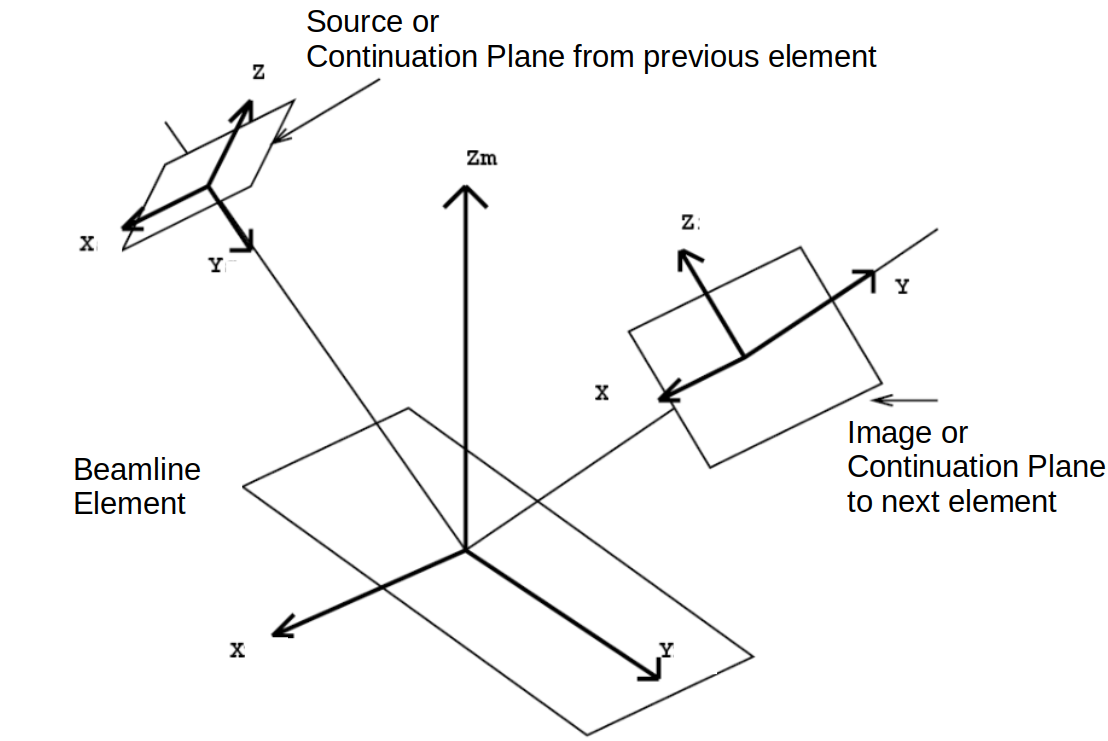
\includegraphics[width=0.9\linewidth]{figures/S4_reference_frame.png}
\caption{SHADOW4 reference frame definitions: Source, beamline element, and image coordinates.}  
\end{figure}

In SHADOW4 the ``beamline element" is formed by an ``optical element" object and a ``coordinates" object containing two angles: the incidence angle $\theta$ and the beamline element orientation angle $\alpha$, and two distances: the distance $p$ from the source (or continuation plane from the previous element), and $q$ from the beamline element to its image plane or continuation plane.
The beamline element orientation angle $\alpha$ is not reset after the scattering in the beamline element (reflection, refraction or diffraction), therefore it influences the orientation of the axis at the image (see Fig.~\ref{fig:S4_orientations}).

\begin{figure}
\label{fig:S4_orientations}
    \centering
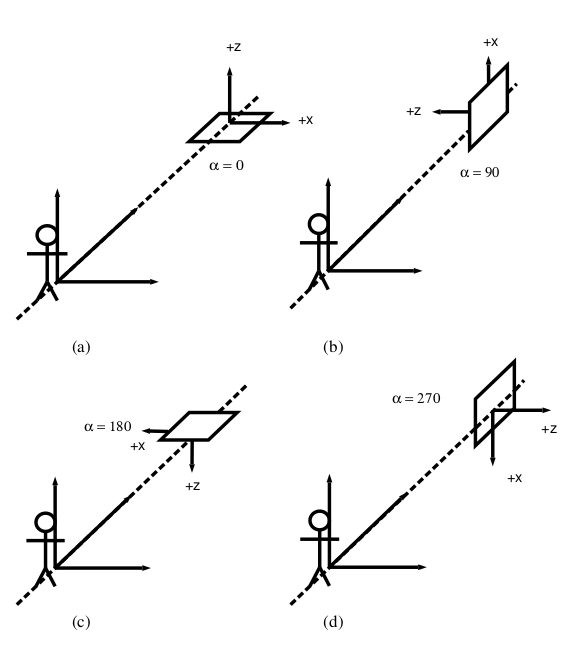
\includegraphics[width=0.9\linewidth]{figures/S4_orientations.png}
\caption{Effect of the beamline element orientation angle $\alpha$ for the four most common values: 0, 90, 180 and 270 degrees. The effect of the angle $\alpha$ is carried out to the image plane, thus defining the position of the axes (in blue). }  
\end{figure}


The beam coming from the source or a previous beamline element must be converted into the reference frame of the o.e. for performing the ray tracing.
The rotation of the vectors of the rays in the beam ($\vec{x}$, $\vec{v}$ and $\vec{E}_{\sigma,\pi}$) around a given axis is done in the method {\tt S4Beam.rotate}\footnote{\tiny \url{https://shadow4.readthedocs.io/en/latest/shadow4.beam.html#shadow4.beam.s4_beam.S4Beam.rotate}}. 
Therefore, to put the beam in the local reference of the beamline element, the beam vectors ($\vec{x}$,  $\vec{v}$ and $\vec{E}_{\sigma,\pi}$) are affected by these sequential operations:
\begin{itemize}
    \item rotate the vectors by an angle $\alpha$ around the $\hat{u}_y$=(0,1,0); 
    \item rotate the vectors by an angle $\theta_i$ around $\hat{u}_x$,
    \item translate the beam coordinates $\vec{x}$ a distance $-p$.
\end{itemize}
As an example, see the listed code\footnote{\tiny \url{https://shadow4.readthedocs.io/en/latest/shadow4.beamline.optical_elements.mirrors.html#shadow4.beamline.optical_elements.mirrors.s4_mirror.S4MirrorElement.trace_beam}}.

Then, the reflection/refraction/diffraction by the beamline element is applied, which changes the beam direction and electric vectors.
This will be discussed in detail in the next paragraphs.

Last, after the reflection, the rays are\footnote{
These operations are done by the method {\tt S4Beam.change\_to\_image\_reference\_system}, see: {\tiny \url{https://shadow4.readthedocs.io/en/latest/shadow4.beam.html#shadow4.beam.s4_beam.S4Beam.change_to_image_reference_system}}.
} 
\begin{itemize}
    \item projected into the image plane, and
    \item change the coordinate system to have the origin in the image plane.
\end{itemize}
For that it projects the  vectors onto the versors of the new reference. 


It is important that the changes of refecence system (before and after interaction with the beamline element)  are not affecting the phase $\phi_\sigma$ and $\phi_\pi$ and conserve the modulus of each electric field component $\vec{E}_\sigma$ and $\vec{E}_\pi$. Also, they do not alter the orthogonality relationships:
\begin{eqnarray}
\label{ortho}
\vec{E}_\sigma \perp \vec{E}_\pi \nonumber \\
\vec{E}_\sigma \perp \vec{v} \nonumber \\
\vec{E}_\pi \perp \vec{v}.
\end{eqnarray}


% -----------------------------------------------------------------
% -----------------------------------------------------------------
\section{Interaction with the beamline element using Jones calculus}
\label{sec:S4}

The interaction of the SHADOW beam with the optical element  uses the Jones calculus \cite{Jones1941a, Jones1941b} in SHADOW4. We explain here the theory and implementation. This is new in SHADOW4, and the old implementation in SHADOW3 is described in Appendix~\ref{sec:S3}.

Fully polarized light can be described using the Jones calculus. The polarized electric field is represented by a Jones vector, made by two complex numbers representing the scalar electric field for the $\sigma$ and $\pi$ polarizations. 
The effect of the beamline elements are represented by Jones matrices.
In such a way, the light after the interaction with the optical element is found by taking the product of the Jones matrix of the optical element and the Jones vector of the incident light.

Jones vector for a ray, following equation~(\ref{eq:electricfieldray2}), is
\begin{equation}
        \begin{pmatrix}
        \mathcal{E}_\sigma \\
        \mathcal{E}_\pi
    \end{pmatrix}
    =
    \begin{pmatrix}
        |\vec{E}_{\sigma}| e^{i \phi_\sigma} \\
        |\vec{E}_{\pi}| e^{i \phi_\pi}
    \end{pmatrix}.
\end{equation}

In general, a Jones matrix is applied to a Jones vector to get the scattered Jones vector
\begin{equation}\label{eq:applyJones}
    \begin{pmatrix}
        \mathcal{E}'_\sigma \\
        \mathcal{E}'_\pi
    \end{pmatrix}
    =
    \textbf{J}
    \cdot
    \begin{pmatrix}
        \mathcal{E}_\sigma\\
        \mathcal{E}_\pi
    \end{pmatrix}.
\end{equation}

The Jones matrix that represents a generic beamline element is\footnote{The off-diagonal elements in the most common beamline elements like crystals, gratings, mirrors and multilayer are zero}
\begin{equation}\label{eq:J}
\textbf{J}_e = 
\begin{pmatrix}
r_{\sigma\sigma} & r_{\sigma\pi}\\
r_{\pi\sigma} & r_{\pi\pi}
\end{pmatrix},
\end{equation}
where the elements are the complex scattering amplitudes.
Note that the $\sigma$ and $\pi$ directions here are ``local" (they are referred to the scattering plane). 
This implies that $\textbf{J}_e$ in equation~(\ref{eq:J}) cannot be directly applied to the Jones vector of the incident ray, but has to be transformed. 

The $\sigma$ and $\pi$ directions of polarization are defined by the scattering plane spanned by the direction vectors before and after the scattering: $\vec{v}$ and $\vec{v}'$, respectively.
It is convinient to consider the $\sigma$ and $\pi$ versors in three different frames, defined:
\begin{itemize}
    \item the $\hat{u}_\sigma$ and $\hat{u}_\pi$ for the incoming ray as defined in equation~(\ref{eq:electricfieldray2}), 

    \item for the scattering plane spanned by $\vec{v}$ (incident direction): 

\begin{eqnarray}\label{eq:u_i}
  \hat{u}_{\sigma,i} 
  &=&
  \frac{\vec{v} \times \vec{v}'}{\left| \vec{v} \times \vec{v}' \right|}
  \nonumber \\
  \hat{u}_{\pi,i}
  &=&
  \frac{\vec{v} \times \hat{u}_{\sigma,i}}{\left| \vec{v} \times \hat{u}_{\sigma,i} \right|}.
\end{eqnarray}

    \item for the scattering plane spanned by $\vec{v}'$ (output or final direction): 

\begin{eqnarray}\label{eq:u_f}
  \hat{u}_{\sigma,f} 
  &=&
  \hat{u}_{\sigma,i} 
  \nonumber \\
  \hat{u}_{\pi,f}
  &=&
  \frac{\vec{v}' \times \hat{u}_{\sigma,f}}{\left| \vec{v}' \times \hat{u}_{\sigma,f} \right|}.
\end{eqnarray}
\end{itemize}
All $\hat{u}$ are real 3D unit vectors.
% Note: Signs or order of the cross products may be chosen differently, depending on how you want to define a right-handed coordinate system with these 3 vectors as basis.
Note that in forward scattering, $\vec{v}' = \vec{v}$, the scattering plane is ill defined, and an arbitrary direction can be chosen (we use $\hat{u}_{\sigma,i}=\hat{u}_{\sigma}$).

The electric vector in the frame related to the diffraction plane (with axes along $\hat{u}_{\sigma,i}$, $\vec{v}$, and $\hat{u}_{\pi,i}$) is expressed as 
\begin{equation}
  \left( \begin{array}{c}
    E_{\sigma,i} e^{i \phi_{\sigma,i}} \\
    E_{\pi,i} e^{i \phi_{\pi,i}}
  \end{array} \right)
  =
  \underbrace{
  \left( \begin{array}{cc}
    \hat{u}_{\sigma,i} \cdot \hat{u}_{\sigma} &
    \hat{u}_{\sigma,i} \cdot \hat{u}_{\pi} \\
    \hat{u}_{\pi,i} \cdot \hat{u}_{\sigma} &
    \hat{u}_{\pi,i} \cdot \hat{u}_{\pi} 
  \end{array} \right)
  }_{\textbf{R}(\alpha)}
  \cdot
  \left( \begin{array}{c}
    E_{\sigma} e^{i \phi_{\sigma}} \\
    E_{\pi} e^{i \phi_{\pi}}
  \end{array} \right).
\end{equation}

The $2\times 2$ matrix is a coordinate transform that can be seen as a rotation

\begin{equation}\label{eq:rotation}
  \textbf{R}(\alpha)
  =
  \left( \begin{array}{cc}
    \cos(\alpha) & -\sin(\alpha) \\
    \sin(\alpha) & \cos(\alpha)
 \end{array} \right)
\end{equation}


% The $\sigma$ direction is coincident with the $x$ axis when the surface normal is along $z$ and the scattering plane is $yz$ (this is the default case). The $\pi$ direction is therefore in the $yz$ plane, and is perpendicular to $\sigma$ and the incident direction $\vec{v}$.

% https://pleclair.ua.edu/optics/Notes/Jones.pdf

% A rotation matrix in 2D transforms the coordinates of a generic point $(x_1,x_2)^T$ into the coordinates $(x'_1,x'_2)^T$ in a new reference system rotated an angle $\phi$ is (see, e.g., \cite{LeClair})
% \begin{equation}
% \textbf{R}(\phi) = 
% \begin{pmatrix}
% \cos\phi & -\sin\phi\\
% \sin\phi & \cos\phi
% \end{pmatrix},
% \end{equation}
% in such a way that
% \begin{equation}
% \begin{pmatrix}
% x'_1 \\
% x'_2
% \end{pmatrix} = 
% \textbf{R}(\phi)
% \begin{pmatrix}
% x_1 \\
% x_2
% \end{pmatrix}.
% \end{equation}

The Jones matrix in equation~(\ref{eq:J}) is now applied to the incident Jones vectors as

\begin{equation}
  \left( \begin{array}{c}
    \mathcal{E}_{\sigma,f} \\
    \mathcal{E}_{\pi,f}
  \end{array} \right)
  =
    \textbf{J}_e \cdot
  \left( \begin{array}{c}
    \mathcal{E}_{\sigma,i} \\
    \mathcal{E}_{\pi,i}
  \end{array} \right)
  =
  \textbf{J}_e \cdot \textbf{R}(\alpha) \cdot
  \left( \begin{array}{c}
    E_{\sigma} e^{i \phi_{\sigma}} \\
    E_{\pi} e^{i \phi_{\pi}}
  \end{array} \right),
\end{equation}
where $\mathcal{E}$ are complex amplitudes along the different direction versors.

% Consider now an incident ray whose electric fields is along the directions $\vec{u}_\sigma$ and $\vec{u}_\pi$. Let be $\alpha$ the angle between $\vec{u}_\sigma$ and $\sigma$ direction of the beamline element  (always perpendicular to the scattering plane). The Jones matrix to be applied to this ray is\footnote{
% In \cite{LeClair} it is said that if an optical element is rotated about the optical axis by an angle $\alpha$, the Jones matrix for the
% rotated element $\textbf{J}_\alpha$ is constructed from the matrix for the unrotated element $\textbf{J}$ by rotating by an angle $\alpha$, applying the matrix $\textbf{J}$, and rotating back by an angle $\-\alpha$:
% $\textbf{J}_\alpha = \textbf{R}(-\alpha) \textbf{J} \textbf{R}(\alpha)$.
% Considering that in SHADOW the rotation of $\alpha$ is not reset, it implies that we must use instead the equation~(\ref{eq:Jalpha_S4}).
% }
% \begin{equation}\label{eq:Jalpha_S4}
%     \textbf{J}_\alpha =  \textbf{J} \textbf{R}(\alpha)=
%     \begin{pmatrix}
% r_\sigma c & -r_\sigma s\\
% r_\pi s& 
% r_\pi c
% \end{pmatrix}.
% \end{equation}
% Therefore, the particular cases for zero and 90$^\circ$ are
% \begin{equation}
% \textbf{J}_{0^\circ} = 
% \begin{pmatrix}
% r_\sigma & 0\\
% 0 & r_\pi
% \end{pmatrix},\text{~and~}
% \textbf{J}_{90^\circ} = 
% \begin{pmatrix}
% 0 & -r_\sigma\\
% r_\pi & 0
% \end{pmatrix}. \nonumber
% \end{equation}
%
% Jones vector $E^J$ for a ray, following Eq.~\ref{eq:electricfieldray}, is
% \begin{equation}
%     E^J = 
%         \begin{pmatrix}
%         e_1 \\
%         e_2
%     \end{pmatrix}
%     =
%     \begin{pmatrix}
%         |E_{\sigma}| e^{i \phi_\sigma} \\
%         |E_{\pi}| e^{i \phi_\pi}
%     \end{pmatrix}.
% \end{equation}

To convert a Jones vector to SHADOW variables we must know the versors with the directions of the electric field.
After scattering of a beamline element, the versors to consider are those of equations~(\ref{eq:u_f}).
Then, $\vec{E}_\sigma=|\mathcal{E}_\sigma| \hat{u}_{\sigma,f}$, and 
$\phi_\sigma=\arg(\mathcal{E}_{\sigma,f})$
(and a similar expression holds for the $\pi$ component).

Note that in the SHADOW implementation, the particular values of $\vec{E}_\sigma$ are correlated to the $\phi_\sigma$ (same for $\pi$): it is always possible to get an equivalent description of the field with $\phi_\sigma$=0. For that, the vectors $\vec{E}_\sigma$ and $\vec{E}_\pi$ are rotated an angle $\phi_\sigma$ around the axis $\vec{v}$ and then the new phases are set to $\phi_\pi \xleftarrow{}(\phi_\pi-\phi_\sigma)$ and $\phi_\sigma\xleftarrow{}0$. In particular, a change of sign in $\vec{E}_\sigma$ corresponds to adding $\pi$ to $\phi_\sigma$.


% In SHADOW4 we calculate the scattering in a beamline element (mirror and multilayer reflections, crystal and grating diffraction, lens refraction) applying the Jones formalist.

In summary, the different steps to be followed in the ray-tracing calculation, considering the input beam already in the local reference of the beamline element (i.e., all the vectors such as direction and electric fields are expressed in the optical element local reference, as described in section~\ref{sec:change_frame}), are:

\begin{enumerate}

\item From every ray we extract the input direction $\vec{v}$, the phases $\phi_{\sigma,\pi}$, and the electric field vectors $\vec{E}_{\sigma,\pi}$. We construct the versor directions $\hat{u}_{\sigma,\pi}$, and the Jones vector $(\mathcal{E}_\sigma, \mathcal{E}_\pi)^T$.

\item From the model of the beamline element we obtain the outgoing direction $\vec{v}'$ (geometrical model), and the reflectivities (physical model) to build $\mathbf{J}_e$ [equation~(\ref{eq:J}))].

\item Construct the versors in equations~(\ref{eq:u_i}) and (\ref{eq:u_f}) and the matrix $\textbf{R}(\alpha)$.


\item Compute the Jones matrix $\textbf{J}_e \cdot \textbf{R}(\alpha)$ [equation~(\ref{eq:rotation})].

\item Calculate the scattered Jones vector using equation~(\ref{eq:applyJones}).

\item Compute the SHADOW variables $\vec{E}'_{\sigma,\pi}$ and $\phi'_{\sigma,\pi}$ for the reflected ray with the amplitudes in the scattered Jones vector $(E^J)'$ and directions $\hat{u}_{\sigma,f}$ and $\hat{u}_{\pi,f}$.
\end{enumerate}



% -----------------------------------------------------------------
% -----------------------------------------------------------------
\section{X-ray polarizers based on crystals with $\theta_B$=$\pi$/4}\label{sec:polarizers45degBenchmark}
% -----------------------------------------------------------------
% -----------------------------------------------------------------

We want to study the polarization produced in an x-ray beam by a series of reflections with $\theta_B=\pi/4$. In this case, the crystal reflectivity (in amplitudes) is $r_\sigma \approx 1$ and $r_\pi \approx 0$. The interest of multiple reflections is to eliminate the $\pi$ component by successive reflections (i.e. multiplication) by $r_\pi$.

\subsection{Benchmarking}

In this paragraph we consider the Si800 crystal that for $\theta_B=45^{\circ}$ the corresponding photon energy is 12914.735~eV. For practical purposes we consider the beam at photon energy 12914~eV. The Bragg angle at this energy is $\theta_B=44.999996^{\circ}$, and the ``corrected Bragg angle" (at which the crystal is positioned) is $\theta_{Bc}=45.000331^{\circ}$.
At this corrected Bragg angle, the reflectivities are $r_\sigma=-0.0247-0.970 i$ and $r_\pi=0.000933+0.001100 i$.
The squared modulus, or reflectance, are $R_\sigma=|r_\sigma|^2=0.941660$ and 
$R_\pi=|r_\pi|^2=2.081562~10^{-06}$.

Let us use 8 crystals, divided in two packs of 4 crystals each (the ``polariser" and the ``analyser"). A pack has the crystals in non-dispersive configuration $(+,-,+,-)$. The second pack is rotated 90$^\circ$ with respect to the first pack. Therefore we consider all the crystals as a single rigid body, with all crystals well aligned.

We now have to define the incident beam and the orientation of the first crystal with respect to this beam. For our first tests we define an idealized pencil beam (zero cross section, and zero divergence), with a given polarization $P$. In our ray tracing source, all rays are identical. We consider two cases that will be referred as case 1 and case 2 respectively:
\begin{enumerate}
    \item a source linearly polarized with $P=1$ (Jones vector of each ray $(1,0)^T$) and first crystal rotated -45$^\circ$ along the beam direction (zero is facing up).
    \item a source linearly polarized with $P=0.5$ [Jones vector of each ray $(2^{-1/2},2^{-1/2})^T$] and first crystal is facing up.    
\end{enumerate}

\subsubsection{Case 1}
The Jones vector of the incident ray is $(1,0)^T$ and first crystal is rotated $\alpha$=-45$^\circ$ (therefore $s=-2^{-1/2}$ and $s=2^{-1/2}$). The Jones matrices of the first crystal is: 
\begin{equation}\label{eq:Jcase1_xtal1_S4}
    \textbf{J}_1=\textbf{J}_e \cdot \textbf{R}(-45^{\circ})
    \cdot
    2^{-1/2}
    \begin{pmatrix}
r_\sigma  &
r_\sigma \\
- r_\pi& 
r_\pi
\end{pmatrix}.
\end{equation}
For the other crystals
\begin{equation}\label{eq:Jcase1_S4}
\textbf{J}_{2,3,4,6,7,8}=
    \begin{pmatrix}
r_\sigma & 0\\
0& 
r_\pi
\end{pmatrix},
\end{equation}
and
\begin{equation}\label{eq:J5case1_S4}
\textbf{J}_{5}=\textbf{J}_e\cdot \textbf{R}(90^{\circ})
=
\begin{pmatrix}
0 & -r_\sigma\\
r_\pi& 0
\end{pmatrix}
\end{equation}

Therefore, the Jones vector after all reflections is:
\begin{equation}\label{eq:JVcase1_S4}
\left[ \prod_{i=1}^{8} \textbf{J}_i \right]
    \cdot
    \begin{pmatrix}
    1\\0
    \end{pmatrix}=
    2^{-1/2} r_\sigma^4 r_\pi^4
        \begin{pmatrix}
   1&-1\\
    1 & 1
    \end{pmatrix}
    \cdot
        \begin{pmatrix}
    1\\0
    \end{pmatrix}
    =
    2^{-1/2}r_\sigma^4 r_\pi^4
    \begin{pmatrix}
    1\\
    1
    \end{pmatrix}.
\end{equation}

The intensities are (for 1000 rays)
\begin{itemize}
    \item $\sigma$-polarized $I_\sigma=|2^{-1/2}~r_\sigma^4 r_\pi^4|^2$=7.38~ 10$^{-21}$
    \item $\pi$-polarized: the same 
    \item total 1.47~ 10$^{-21}$.
\end{itemize}
SHADOW4 rasults are in good agreement.

\subsubsection{Case 2}

The Jones vector of the incident ray is $(2^{-1/2},2^{-1/2})^T$.
The Jones matrices are: 
\begin{equation}\label{eq:Jcase2_S4}
\textbf{J}_{1,2,3,4,6,7,8}=
    \begin{pmatrix}
r_\sigma & 0\\
0& 
r_\pi
\end{pmatrix}
\end{equation}
and
\begin{equation}\label{eq:J5case2_S4}
\textbf{J}_{5}=\textbf{J}_e \cdot \textbf{R}(90^\circ)=
\begin{pmatrix}
0 & -r_\sigma\\
r_\pi& 0
\end{pmatrix}
\end{equation}

Therefore, the Jones vector after all reflections is:
\begin{equation}\label{eq:JVcase2_S4}
\left[ \prod_{i=1}^{8} \textbf{J}_i \right]
    \cdot 
    \begin{pmatrix}
    2^{-1/2}\\2^{-1/2}
    \end{pmatrix}=
    r_\sigma^4 r_\pi^4
        \begin{pmatrix}
    0&-1\\
    1 & 0
    \end{pmatrix}
    \cdot
        \begin{pmatrix}
    2^{-1/2}\\2^{-1/2}
    \end{pmatrix}
    =
    2^{-1/2}r_\sigma^4 r_\pi^4
    \begin{pmatrix}
    -1\\
    1
    \end{pmatrix}.
\end{equation}

The intensities are the same as for case 1, and also here SHADOW4 results agree well. 

\subsection{A practical case}\label{sec:polarizers45degPractical}

For an X-ray beam within a polarizer utilizing multiple consecutive reflections in channel-cut crystals with a scattering angle of $2\theta_B$=90$^\circ$, despite each reflection yielding a $\pi$-polarization reflectivity of $r_\pi\approx 0$, achieving perfect linear polarization is not feasible for a divergent beam.
Even with an ideal polarizer, the achievable limit for linear polarization purity is governed by (Schulze, 2018)
\begin{equation}\label{eq:polarizer}
    P = \sigma_h^2 + \sigma_v^2,
\end{equation}
where $\sigma_{h,v}$ are the rms angular divergences in horizontal and vertical directions incidence on polarizer.

We demonstrate a practical example as shown in Fig~1 in ref (Schulze et al., 2022), not only verify the linear purity can be reached by this setting, but also the validity of equation (\ref{eq:polarizer}).

An X-ray source before the polarizer is created with rms divergence parameters of $\sigma_h$=\SI{273}{\nano\radian} and $\sigma_v$=0.
The photon energy is \SI{6457}{eV} (0.01\% bandwidth), and the polarizer and analyser are using channel cut crystals Si400.
$\sigma_h$ is much smaller than the Darwin-width of \SI{26}{\micro\radian} of Si400 at \SI{6457}{eV}.

To simulate the linear purity, the analyser (crystals 5 to 8) is rotated with respect to the primary beam direction after the polariser (crystals 1 to 4) an angle of 0 or 90$^\circ$ to set parallel or crossed to the polarizer, then calculating the ray-tracing intensities $I_\text{parallel}$ and $I_\text{cross}$ at the detector downstream from the analyser, for parallel and crossed setting respectively.
Then the actual linear purity achieved by these polarizer and analyser pair is expressed as $I_\text{cross}/I_\text{parallel}$.

A number of 250K rays are generated at the source, the intensities are $I_\text{parallel}=22348.6$ \inred{(BEFORE: 22173.3)} and $I_\text{cross}=1.667~\times~10^{-9}$ \inred{BEFORE: 1.63$~\times~10^{-9}$}.
Their ratio gives a linear purity of $P=7.46~\times~10^{-14}$ \inred{BEFORE: 7.35$~\times~10^{-14}$}, which agrees very well the prediction value by equation (\ref{eq:polarizer}) of $P=7.45~\times~10^{-14}$.

In the simulation above, we assumed that the electric vector at the source lies in the horizontal plane, with the polarizer’s crystal plane oriented upwards.
For a vacuum birefringence experiment, to achieve the required 45$^\circ$ linear polarization instead of horizontal polarization as specified by \cite{Shen2018}, the polariser has to be rotated 45$^\circ$ around the primary beam direction.
This rotation introduces an additional 50\% intensity loss compared to the previous, unrotated setup.
This loss occurs because half of the beam’s intensity projected onto the crystal’s incident plane is suppressed due to diminished reflectivity of the $\pi$-polarized component.

\begin{figure}\label{fig:polarizer}
\centering
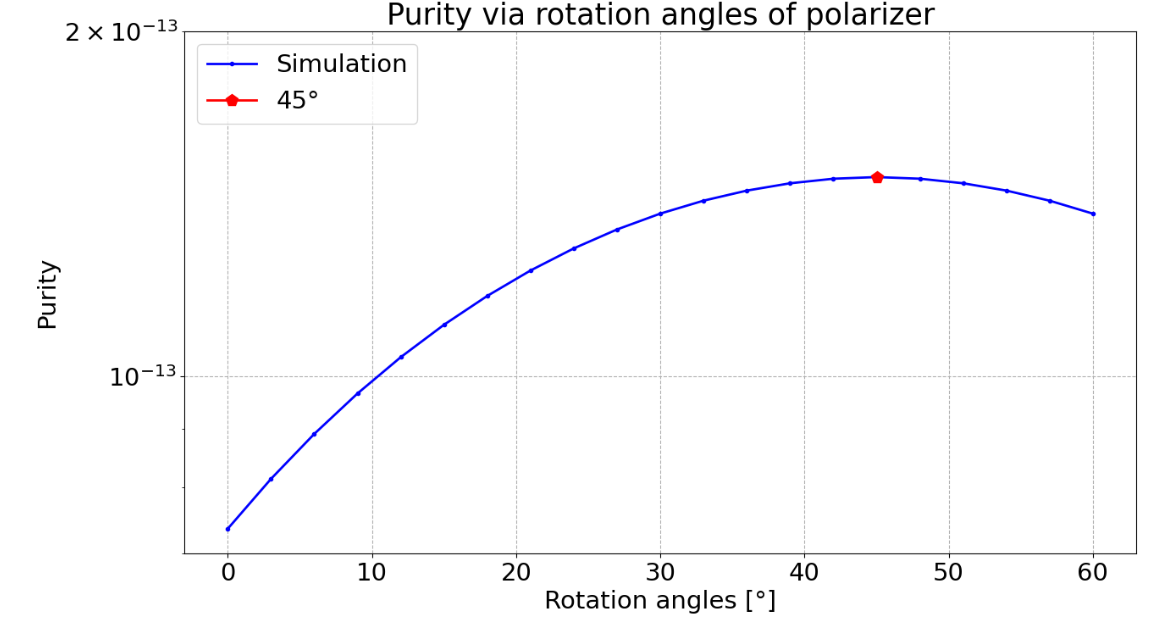
\includegraphics[width=0.95\linewidth]{figures/polarizer.png}
\caption{The linear purity simulation for polariser rotation in angular range of 0 to 60 degrees (legend: Simulation), and the calculation value with equation~(\ref{eq:polarizer}) at 45$^\circ$.}
\end{figure}

The simulated intensity of  $I_\text{parallel}$ aligns well with expectations, showing a reduction to half of its original value without polarizer rotation.
However, the simulated $I_\text{cross}$ intensity remains largely unchanged, thereby doubling the linear polarization purity to 1.5$~\times~10^{-13}$, as shown in Fig.~\ref{fig:polarizer}.
Generally, when rotating the polarizer across a range from 0 to 60$^\circ$, purity values vary, starting at 7.35$~\times~10^{-14}$ at 0, increasing and then decreasing after reaching a peak of 1.5$~\times~10^{-13}$ at 45$^\circ$.
This trend suggests that equation (\ref{eq:polarizer}) holds only for a polarizer orientation of 0 and does not align with simulation data at other angles in the case of an asymmetric angular source, with Gaussian divergence in the horizontal and collimation in the vertical direction.

% -----------------------------------------------------------------
% -----------------------------------------------------------------
\section{Crystal phase-shifters}\label{sec:phasesifters}
% -----------------------------------------------------------------
% -----------------------------------------------------------------

\cite{Bouchenoire2003}
\cite{Bouchenoire2012}
\cite{Detlefs2012}
\cite{Suzuki2023} 

Beamlines: \cite{Francoual2013} \cite{Freeland2002} \cite{Suzuki2014}

% -----------------------------------------------------------------
% -----------------------------------------------------------------
\section{Polarization effects in mirror reflections}\label{sec:phasesifters}
% -----------------------------------------------------------------
% -----------------------------------------------------------------

\cite{Nayar1997}

% -----------------------------------------------------------------
% -----------------------------------------------------------------
\section{Summary and conclusions}
\label{sec:summary}
% -----------------------------------------------------------------
% -----------------------------------------------------------------

zzzzzzz


% %%%%%%%%%%%%%%%%%%%%%%%%%%%%%%%%%%%%%%%%%%%%%%%%
% %%%%%%%%%%%%%%%%%%%%%%%%%%%%%%%%%%%%%%%%%%%%%%%%

\appendix
%\section{Appendix title}

% -----------------------------------------------------------------
% -----------------------------------------------------------------
\section{Interaction with the beamline element (like in SHADOW3)}
\label{sec:S3}
% -----------------------------------------------------------------
% -----------------------------------------------------------------

The effect of the beamline element (reflection/refraction/diffraction) is applied to the beam. In SHADOW3, once the beam arrives to the element, the changes are done in three steps 
\begin{enumerate}
    \item change the incoming electric vectors to the local $\sigma$ and $\pi$ directions.
    \item multiplication of the electric fields by the reflectivities $R_\sigma$ and $R_\pi$ and change the phases accordingly.
    \item modify the outcoming electric field to guarantee the orthogonality with the output (reflected/refracted/diffracted) direction.
\end{enumerate}

% -----------------------------------------------------------------
\subsection{Modifications of electric fields in ``local'' o.e.}
\label{sec:localoe}
% -----------------------------------------------------------------
% -----------------------------------------------------------------


The physics of the X-ray reflection and diffraction in an optical surface affects in a different way 
the {\it local} parallel ($\sigma$) and perpendicular ($\pi$) components. The ``local'' parallel component
is a vector that sits on the o.e. surface and it is not coincident with the incident $\vec{E}_\sigma$.
Therefore, one must calculate the ``local'' $\vec{u}'_\sigma$ and $\vec{u}'_\pi$ vectors that verify
1) they are orthogonal to $\vec{v}$ and ii) $\vec{u}'_\sigma$ is contained in the o.e. surface. 
This is done in the method {\tt get\_local\_directions\_sigma\_pi} of {\tt S4Beam} (listing~\ref{lst:localsigmaandpi}).

% \begin{lstlisting}[caption={Method of {\tt S4Beam} to compute the local directions $\sigma$ and $\pi$ at the beamline element.}, label={lst:localsigmaandpi}, captionpos=b]
%     def get_local_directions_sigma_pi(self, vNormal, vIn=None):
%         """
%         Given a direction N (normal to a surface), this routine calculates the "local sigma and pi"
%         directions, or the unitary vectors perpendicular and parallel to the scattering plane, respectively.
%         The scattering plane is defines as the plane that contains N and the ray direction vIn.

%         Parameters
%         ----------
%         vNormal: numpy array
%             An array of vectors (npoints, 3) with the normal N.
%         vIn: numpy array, optional
%             The array of vectors with the incident direction. If None, it uses the direction in the S4Beam.

%         Returns
%         -------
%             tuple:
%             (direction_sigma, direction_pi) the two unitary array of vectors with the sigma and pi-directions.
%         """
%         if vNormal.shape[1] != 3:
%             raise Exception("vNormal must be an array of vectors (npoints, 3).")

%         if vIn is None: vIn = self.get_columns([4, 5, 6]).T

%         E_S = self.get_columns([7, 8, 9]).T
%         E_P = self.get_columns([16, 17, 18]).T

%         # ! * ... we have to compute
%         # ! * some angles, namely the sine of the incidence angle and the sine
%         # ! * of the A vector with the normal. Also, the polarized light is
%         # ! * treated as a superposition of two orthogonal A vectors with the appropriate
%         # ! * phase relation. These two incoming vectors have to be resolved into the
%         # ! * local S- and P- component with a new phase relation.
%         # ! * A_VEC will be rotated later, once the amplitude will have been determined.
%         #      	CALL	CROSS 	(VVIN,VNOR,AS_TEMP)	! vector pp. to inc.pl.
%         #      	IF (M_FLAG.EQ.1) THEN
%         # 	        CALL	DOT	(AS_VEC,AS_VEC,AS2)
%         # 	        CALL	DOT	(AP_VEC,AP_VEC,AP2)
%         # 	        IF (AS2.NE.0)	THEN
%         #              	 DO 499 I=1,3
%         #  499   	            AS_TEMP(I) = AS_VEC(I)
%         # 	        ELSE
%         # 	             DO 599 I=1,3
%         #  599	            AS_TEMP(I) = AP_VEC(I)
%         # 	        END IF
%         #      	END IF
%         #      	CALL	NORM  	(AS_TEMP,AS_TEMP)	! Local unit As vector
%         # CALL	CROSS	(AS_TEMP,VVIN,AP_TEMP)
%         # CALL	NORM	(AP_TEMP,AP_TEMP)	! Local unit Ap vector

%         v_S = vector_cross(vIn, vNormal)  # AS_TEMP
%         v_Smod = vector_modulus(v_S)
%         mask = (v_Smod == 0.0)
%         if mask.any():
%             print(">>>>>>>>>> FOUND A ZERO!!!!!")
%             if v_Smod.sum() > 0:
%                 v_S[mask, 0] = E_S[mask, 0]
%                 v_S[mask, 1] = E_S[mask, 1]
%                 v_S[mask, 2] = E_S[mask, 2]
%             else:
%                 v_S[mask, 0] = E_P[mask, 0]
%                 v_S[mask, 1] = E_P[mask, 1]
%                 v_S[mask, 2] = E_P[mask, 2]

%         v_P = vector_cross(v_S, vIn)
%         uS = vector_norm(v_S)
%         uP = vector_norm(v_P)

%         return vector_norm(v_S), vector_norm(v_P)
% \end{lstlisting}




The electric vector can thus be expressed in two orthonormal vectors $\vec{E'}_\sigma$ and $\vec{E'}_\pi$ along these 
new directions $\vec{u'}_\sigma$ and $\vec{u'}_\pi$. Physically, it is a rotation of the old electric vectors around
the $\vec{v}$ direction to put the $\sigma$ component on top of the surface, but the rotation affect not only the 
moduli, but also the phases. The new (complex) electric vectors are build from the projection of the old ones onto the
new axes, thus originating a transformation in both moduli and phases:

\begin{eqnarray}
\vec{E'}_\sigma e^{i \phi'_\sigma} = [(\vec{E}_\sigma e^{i \phi_\sigma}).\vec{u'}_\sigma + (\vec{E}_\pi e^{i \phi_\pi}).\vec{u'}_\sigma ] 
  ~~\vec{u'}_\sigma  \\ 
\vec{E'}_\pi e^{i \phi'_\pi} = [(\vec{E}_\sigma e^{i \phi_\sigma}).\vec{u'}_\pi + (\vec{E}_\pi e^{i \phi_\pi}).\vec{u'}_\pi ] 
  ~~\vec{u'}_\pi 
\end{eqnarray}


Defining the projection of the (real) electric field components onto these versors as: 
\begin{eqnarray}
a_{11} = \vec{E}_\sigma . \vec{u'}_\sigma, ~~~~ 
a_{12} = \vec{E}_\inred{\pi} . \vec{u'}_\inred{\sigma} \nonumber \\
a_{21} = \vec{E}_\inred{\sigma} . \vec{u'}_\inred{\pi}, ~~~~
a_{22} = \vec{E}_\pi . \vec{u'}_\pi 
\end{eqnarray}

we get:
\begin{eqnarray}
\label{withphases}
\vec{E'}_\sigma e^{i \phi'_\sigma} = (a_{11} e^{i \phi_\sigma} + a_{12} e^{i \phi_\pi}) \vec{u'}_\sigma \nonumber \\ 
\vec{E'}_\pi e^{i \phi'_\pi} =    (a_{21} e^{i \phi_\sigma} + a_{22} e^{i \phi_\pi}) \vec{u'}_\pi
\end{eqnarray}

And the moduli are: 

\begin{eqnarray}
|\vec{E'}_\sigma|^2 = \vec{E'}_\sigma . \vec{E'}_\sigma^*  = 
a_{11}^2 + a_{12}^2 + 2 a_{11} a_{12} \cos(\phi_\sigma-\phi_\pi) \equiv
M_\sigma^2 \nonumber \\ 
|\vec{E'}_\pi|^2    = \vec{E'}_\pi    . \vec{E'}_\pi^*     = 
a_{21}^2 + a_{22}^2 + 2 a_{21} a_{22} \cos(\phi_\sigma-\phi_\pi) \equiv
M_\pi^2
\end{eqnarray}

Therefore we can construct the new local (real) electric fields as: 
\begin{eqnarray}
\label{final1}
\vec{E'}_\sigma = M_\sigma \vec{u'}_\sigma  \nonumber \\ 
\vec{E'}_\pi = M_\pi \vec{u'}_\pi  
\end{eqnarray}

To compute the new phases, we insert Eq.~\ref{final1} in Eq.~\ref{withphases} and get: 
\begin{eqnarray}
e^{i \phi'_\sigma} = M_\sigma^{-1} (a_{11} e^{i \phi_\sigma} + a_{12} e^{i \phi_\pi})  \nonumber \\ 
e^{i \phi'_\pi} =  M_\pi^{-1}      (a_{21} e^{i \phi_\sigma} + a_{22} e^{i \phi_\pi}) 
\end{eqnarray}

Therefore:
\begin{eqnarray}
\label{final2}
\tan{\phi'_\sigma} = \frac{Im(a_{11} e^{i \phi_\sigma} + a_{12} e^{i \phi_\pi})}
                          {Re(a_{11} e^{i \phi_\sigma} + a_{12} e^{i \phi_\pi})} = 
                          \frac{a_{11} \sin{\phi_\sigma} + a_{12} \sin{\phi_\pi}}
                               {a_{11} \cos{\phi_\sigma} + a_{12} \cos{\phi_\pi}}  \nonumber \\ 
\tan{\phi'_\pi} =  \frac{Im(a_{21} e^{i \phi_\sigma} + a_{22} e^{i \phi_\pi})}
                        {Re(a_{21} e^{i \phi_\sigma} + a_{22} e^{i \phi_\pi})} = 
                        \frac{a_{21} \sin{\phi_\sigma} + a_{22} \sin{\phi_\pi}}
                             {a_{21} \cos{\phi_\sigma} + a_{22} \cos{\phi_\pi}}
\end{eqnarray}


The code that implements Eq.~\ref{final1} and Eq.~\ref{final2} is in listing~\ref{lst:rotationelements}: 

% \begin{lstlisting}[caption={Code to compute the local $\sigma$ and $\pi$ electric fields at the beamline element.}, label={lst:rotationelements}, captionpos=b]
%             #
%             # STEP 1: get local sigma and pi directions v_S and v_P (uS and uP unitary vectors)
%             #

%             uS, uP = footprint.get_local_directions_sigma_pi(vH, vIn=vIn)

%             #
%             # calculate the electric field in the local coordinate system
%             #

%             # CALL	DOT	(AS_VEC,AS_TEMP,A11)	! matrix element of rotation
%             # CALL	DOT	(AP_VEC,AS_TEMP,A12)	! matrix element of rotation
%             # CALL	DOT	(AS_VEC,AP_TEMP,A21)	! matrix element of rotation
%             # CALL	DOT	(AP_VEC,AP_TEMP,A22)	! matrix element of rotation
%             # ! ** Now recompute the ampltitude and phase of the local S- and P- component.
%             # AS_NEW	= SQRT(ABS(A11**2 + A12**2 +  &
%             #         2.0D0*A11*A12*COS(PHS-PHP)))
%             # AP_NEW	= SQRT(ABS(A21**2 + A22**2 +  &
%             #         2.0D0*A21*A22*COS(PHS-PHP)))
%             # CALL	SCALAR	(AS_TEMP,AS_NEW,AS_VEC)	! Local As vector
%             # CALL	SCALAR	(AP_TEMP,AP_NEW,AP_VEC)	! Local Ap vector
%             # PHTS	= A11*SIN(PHS) + A12*SIN(PHP)
%             # PHBS	= A11*COS(PHS) + A12*COS(PHP)
%             # PHTP	= A21*SIN(PHS) + A22*SIN(PHP)
%             # PHBP	= A21*COS(PHS) + A22*COS(PHP)
%             # CALL	ATAN_2	(PHTS,PHBS,PHS)		! Phase of local As vector
%             # CALL	ATAN_2	(PHTP,PHBP,PHP)		! Phase of local Ap vector
%             # ! C
%             # ! C
%             # CALL	DOT	(VVIN,VNOR,SIN_VAL)	! sin(graz. ang)
%             # CALL	DOT	(Q_OUT,VNOR,SIN_REF)	! sin(graz.ref.ang)

%             a11 = vector_dot(E_S, uS)
%             a12 = vector_dot(E_P, uS)
%             a21 = vector_dot(E_S, uP)
%             a22 = vector_dot(E_P, uP)

%             M2_S = a11 ** 2 + a12 ** 2 + 2 * a11 * a12 * numpy.cos(PhiS - PhiP)
%             M2_P = a21 ** 2 + a22 ** 2 + 2 * a21 * a22 * numpy.cos(PhiS - PhiP)

%             E_local_S = vector_multiply_scalar(uS, numpy.sqrt(M2_S))
%             E_local_P = vector_multiply_scalar(uP, numpy.sqrt(M2_P))

%             local_PhiS = numpy.arctan2((a11 * numpy.sin(PhiS) + a12 * numpy.sin(PhiP)) , (a11 * numpy.cos(PhiS) + a12 * numpy.cos(PhiP)))
%             local_PhiP = numpy.arctan2((a21 * numpy.sin(PhiS) + a22 * numpy.sin(PhiP)) , (a21 * numpy.cos(PhiS) + a22 * numpy.cos(PhiP)))
%             # END OF STEP 1
% \end{lstlisting}



Note that these transformations imply a polarization mixing, or not conservation of the intensity of each component during the projection ($|\vec{E'}_\sigma| \ne |\vec{E}_\sigma|$),
but the total intensity is conserved ($I=|\vec{E}_\sigma|^2+|\vec{E}_\pi|^2=
|\vec{E'}_\sigma|^2+|\vec{E'}_\pi|^2$). The phases also change.
% but the difference of thase is conserved $\Phi=\phi_\sigma-\pi_\pi=\phi'_\sigma-\phi'_\pi$ (I think, but I have not demostrated it).
The new electric vectors are orthogonal to $\vec{v}$ by constructions.

% -----------------------------------------------------------------
\subsection{Reflection/refraction in the o.e. and subsequent changes in electric vectors}
\label{sec:reflection}
% -----------------------------------------------------------------

Once the electric vectors are expressed in the o.e. local coordinates ($\vec{E'}_\sigma$ and 
$\vec{E'}_\pi$) they are multiplied by the mirror/crystal reflectivities and the phases also affected: : 
\begin{eqnarray}
 \label{reflectivities}
 \vec{E'}_\sigma^{new} = \vec{E'}_\sigma R_\sigma, \nonumber \\
 \vec{E'}_\pi^{new} = \vec{E'}_\pi R_\pi, \nonumber \\
 {\phi '}_\sigma^{new} = {\phi '}_\sigma + \Sigma_\sigma, \nonumber \\
 {\phi '}_\pi^{new} = {\phi '}_\pi + \Sigma_\pi,
\end{eqnarray}
where $R_\sigma$ and $R_\pi$ are the o.e. reflectivities and $\Sigma_\sigma$ and $\Sigma_\pi$ are the  phases added in the reflection/refraction/diffraction. 

% -----------------------------------------------------------------
\subsection{subsequent changes in electric vectors to guarantee orthogonality}
\label{sec:orthogonality}
% -----------------------------------------------------------------

The resulting electric vectors and phases after applying Eq.~\ref{reflectivities} must now hold the orthogonality relations (Eq.~\ref{ortho}) with respect to the new direction $\vec{v'}$, therefore they must be changed. 

% \color{red}
% This part was incorrectly
% done in the following code, which assumes conservation of the $\vec{E'}_\sigma$ component (except for gratings)
% and the $\pi$ component is ``mirrored''. These operations do not garantee that the resulting 
% vectors are normal to $\vec{v'}$. In some cases, in particular for $\sigma$ polarizad light onto 
% o.e.'s with mirror orientation angle $90^\circ$ can result in a loss of beam intensity in 
% subsequent changes of frames. The {\bf wrong} code was (in {\tt MIRROR1}): 
% \color{black}

% \begin{lstlisting}
% ! ** So far we have the new amplitude of the two components. We have now
% ! ** to 'reflect' A_VEC onto the mirror. For this, notice that the s-comp
% ! ** is geometrically unchanged, while the p-comp is changed. The angles
% ! ** are exchanged with respect to VVIN. Things are more complicated in
% ! ** the case of a grating, due to the vectorial nature of the diffraction,
% ! ** not treated here. We make the simplifying assumption that the
% ! ** diffraction will not change the degree of polarization. This mean that
% ! ** A_VEC will have the same components referred to the ray as before the
% ! ** diffraction. 

% VVOUT(1)	=   RAY(4,ITIK)
% VVOUT(2)	=   RAY(5,ITIK)
% VVOUT(3)	=   RAY(6,ITIK)
% ! C 
% ! C The following IF block applies only to the GRATING case.
% ! C The binormal is redefined in terms of the diffraction
% ! C plane.
% ! C
%      	IF (F_GRATING.NE.0.OR.F_BRAGG_A.EQ.1) THEN
% 	  CALL	PROJ	(VVOUT,VNOR,VTEMP)
% 	  CALL	SCALAR	(VTEMP,-2.0D0,VTEMP)
% 	  CALL	SUM	(VTEMP,VVOUT,VTEMP)
% 	  !CALL	CROSS	(VTEMP,VNOR,AS_TEMP)
% 	  CALL	CROSS_M_FLAG	(VTEMP,VNOR,AS_TEMP,M_FLAG)
%      	 IF (M_FLAG.EQ.1) THEN
% 	   CALL	DOT	(AS_VEC,AS_VEC,AS2)
% 	   CALL	DOT	(AP_VEC,AP_VEC,AP2)
% 	  IF (AS2.NE.0)	THEN
%      	    DO 899 I=1,3
%  899          AS_TEMP(I) = AS_VEC(I)
% 	  ELSE
% 	   DO 999 I=1,3
%  999	     AS_TEMP(I) = AP_TEMP(I)
%      	  END IF
% 	 END IF
%      	  CALL	NORM  	(AS_TEMP,AS_TEMP)	! Local unit As vector
% 	  CALL	CROSS	(AS_TEMP,VTEMP,AP_TEMP)
% 	  CALL	NORM	(AP_TEMP,AP_TEMP)	! Local unit Ap vector
%      	  CALL	DOT	(AS_VEC,AS_VEC,RES)
%      	  RES	=    SQRT (RES)

%      	  CALL	SCALAR	(AS_TEMP,RES,AS_VEC)
% 	  CALL	DOT	(AP_VEC,AP_VEC,RES)
% 	  RES	=    SQRT (RES)
% 	  CALL	SCALAR	(AP_TEMP,RES,AP_VEC)
%      	END IF


% CALL	PROJ	(AP_VEC,VNOR,VTEMP)
% CALL	VECTOR	(VTEMP,AP_VEC,VTEMP)
% CALL	SCALAR	(VTEMP,-2.0D0,VTEMP)

% CALL	SUM	(AP_VEC,VTEMP,AP_VEC)
% \end{lstlisting}

% \color{red}

The code simply calculates the new $\sigma$ and $\pi$ versors orthogonal to $\vec{v'}$ and affects them by the electric field moduli that do not change. 
Also, the phases are not changed. 
This guarantees that the intensity is conserved, as well as orthogonality.
The code is in listing~\ref{lst:finalorthogonality}: 


% \color{black}

% \begin{lstlisting}[caption={\todo{CORRECT!!} Code to guarantee that the local $\sigma$ and $\pi$ electric fields hold the orthogonality relationships.}, label={lst:finalorthogonality}, captionpos=b]
%             #
%             # STEP 3
%             #

%             # ! Electric vectors are changed to assure orthogonality with the new direction VVOUT
%             # ! To conserve intensity, the moduli of Es and Ep must not change
%             # ! AS_VEC and VVOUT are not orthogonal so a projection of S and P coordinates into the
%             # ! new ones do not work as it may be a component of the electric field along VVOUT
%             #
%             # CALL CROSS_M_FLAG  (VVOUT,VNOR,AS_TEMP,M_FLAG) ! vector pp. to inc.pl.
%             # CALL DOT (AS_VEC,AS_VEC,AS2)
%             # CALL DOT (AP_VEC,AP_VEC,AP2)
%             #
%             # IF (M_FLAG.EQ.1) THEN
%             #  IF (AS2.NE.0) THEN
%             #    DO I=1,3
%             #      AS_TEMP(I) = AS_VEC(I)
%             #    END DO
%             #  ELSE
%             #   DO I=1,3
%             #    AS_TEMP(I) = AP_VEC(I)
%             #   END DO
%             #  END IF
%             # END IF
%             #
%             # CALL NORM   (AS_TEMP,AS_TEMP) ! Local unit As vector perp to vvout
%             # CALL CROSS (AS_TEMP,VVOUT,AP_TEMP)
%             # CALL NORM (AP_TEMP,AP_TEMP) ! Local unit Ap vector perp to vvout
%             #
%             # do i=1,3
%             #   as_vec(i) = as_temp(i) * sqrt(as2)
%             #   ap_vec(i) = ap_temp(i) * sqrt(ap2)
%             # end do

%             aS = vector_modulus(E_diffracted_S)
%             aP = vector_modulus(E_diffracted_P)

%             v_S = vector_cross(vOut, vH) # AS_TEMP
%             v_Smod = vector_modulus(v_S)
%             mask = (v_Smod == 0.0)
%             if mask.any():
%                 print(">>>>>>>>>> FOUND A ZERO!!!!!")
%                 if v_Smod.sum() > 0:
%                     v_S[mask, 0] = E_diffracted_S[mask, 0]
%                     v_S[mask, 1] = E_diffracted_S[mask, 1]
%                     v_S[mask, 2] = E_diffracted_S[mask, 2]
%                 else:
%                     v_S[mask, 0] = E_diffracted_P[mask, 0]
%                     v_S[mask, 1] = E_diffracted_P[mask, 1]
%                     v_S[mask, 2] = E_diffracted_P[mask, 2]

%             v_P = vector_cross(v_S, vOut) # AP_TEMP

%             uS = vector_norm(v_S)
%             uP = vector_norm(v_P)

%             E_diffracted_S[:, 0] = uS[:, 0] * aS
%             E_diffracted_S[:, 1] = uS[:, 1] * aS
%             E_diffracted_S[:, 2] = uS[:, 2] * aS

%             E_diffracted_P[:, 0] = uP[:, 0] * aP
%             E_diffracted_P[:, 1] = uP[:, 1] * aP
%             E_diffracted_P[:, 2] = uP[:, 2] * aP

%             # END STEP 3
% \end{lstlisting}

%%%%%%%%%%%%%%%%%%%%%%

\newpage
\referencelist{iucr}


\end{document}                    % DO NOT DELETE THIS LINE
%%%%%%%%%%%%%%%%%%%%%%%%%%%%%%%%%%%%%%%%%%%%%%%%%%%%%%%%%%%%%%%%%%%%%%%%%%%%%%
